%______________________________________________________________________________
% main.tex

\input{preamble12-screen.tex}
\hypersetup{%
    pdfauthor={Mike Pierce}%
   ,pdftitle={Math N16B Homework Three, Summer 2021}%
   ,pdfkeywords={Pierce,MathN16B,16B,N16B,Calculus,Integration,Berkeley}%
}
\usepackage{fourier}
\input{accessible-colors.tex}
\input{newcommand.tex}
\input{newenvironment.tex}
\pagestyle{empty}


\begin{document}

\begin{center}
    {\Huge{Homework Three}}
    \\ \footnotesize{Analytic Geometry and Calculus}
    \\ \footnotesize{UC Berkeley Math N16B, Summer 2021}
\end{center}
\vspace{2em}

Upload your responses to the prompts marked
(\textsc{\textcolor{magenta}{Submit}})
to Gradescope before 8pm Friday; 
you will receive feedback on these.
\begin{center}
    \href{https://www.gradescope.com/courses/275664}%
    {\texttt{gradescope.com/courses/275664}}
\end{center}
The rest of the exercises you should complete at your discretion.
Note that \emph{Calculus with Applications, 11th Edition} 
has some select solutions, usually to odd-numbered exercises, in the back.


\section*{Goals this Week}

Here are some goals you should have in mind while exercising:
\begin{enumerate}
    \item 
        Learn to feel comfortable plotting multi-variable equations. 
        There is no \emph{procedure} for doing this.
        It's an art. You've got to feel comfortable investigating an equation,
        looking at its level curves, plotting points, etc. 
        Note though that you're only doing this to appreciate the art of it;
        in practice you just use computer software.
    \item 
        Become proficient calculating partial derivatives.
    \item
        Understand what a partial derivative \emph{is}.
        Like, basically you should understand how your intuition 
        for the derivative of a function as a rate of change (slope)
        fits into the context of multivariable functions.
\end{enumerate}

\newpage

\section*{Exercises}

\begin{enumerate}
    \item % 
        I expect that you should be able to (1) accurately 
        evaluate a multi-valued function at a set of values and 
        (2) graph a plane in three-dimensional space.
        From Chapter 9.1 of \emph{Calculus with Applications, 11th Edition}
        work through the enough of the initial exercises 
        that you can do these things.
        Then consider these exercises too:
        \begin{center}
            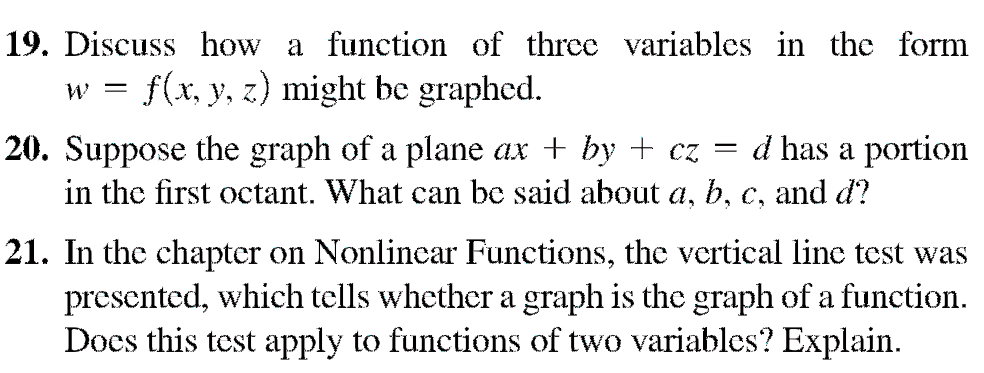
\includegraphics[width=.83\textwidth]{screenshots/192021.png}
        \end{center}
        \begin{center}
            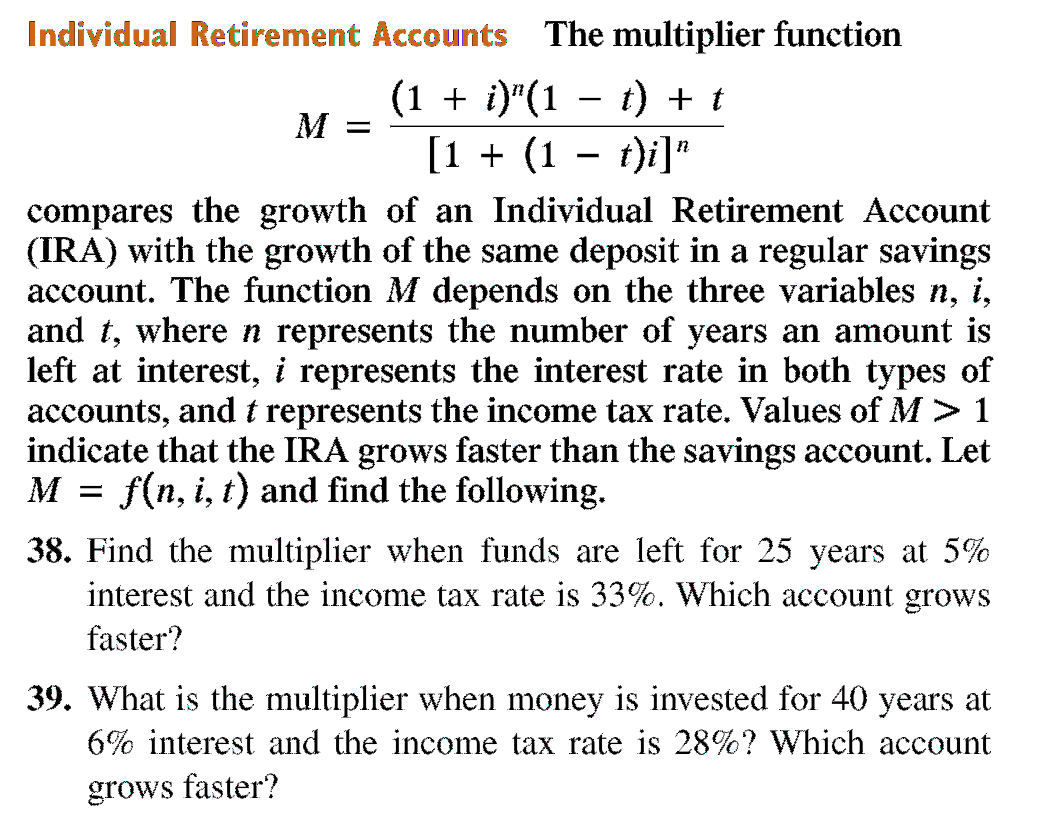
\includegraphics[width=.83\textwidth]{screenshots/3839.png}
        \end{center}

    \item 
        (\textsc{Individual Retirement Accounts})
        That previous example I screenshot from the textbook 
        is stupid for a couple of reasons, but the major reason
        is that \emph{the interest rate on an IRA and on a savings account
        are vastly different}! Ie, the $i$ in the numerator and 
        denominator of $M$ should be different parameters.
        This is because your IRA derives its value from stocks,
        bonds, mutual funds, etc, whereas the interest 
        on your savings account is a pittance the bank gives you,
        probably only because they're legally required to do so.
        Look up the typical annual returns on an IRA 
        (or an analogous long-term retirement account if you're outside the US)
        and the interest rate of a typical bank savings account
        (or use the interest rate on your own savings account if you have one),
        and use these honest values 
        to answer the questions in the screenshot above again.

        That example is also stupid because it assumes the tax rate $t$ 
        is some constant over the $n$ years that you stay invested.
        But again, the $t$ in the numerator and denominator 
        shouldn't even be the same parameter!
        For a normal IRA you only pay taxes once you start withdrawing money
        from the account, so the $t$ in the numerator should be the tax rate
        \emph{after you've been invested for $n$ years},
        whereas the $t$ in the denominator is a function of time
        since you started the account. 
        If however you have a Roth IRA,
        you pay taxes putting money into the account
        so in this case these should at least be the function of $t$
        in the numerator and denominator of $M$.
        ... There is no question here. I just think it's important 
        that, when you're handed an equation and told ``\emph{this 
        equation models this thing,}'' that you contemplate 
        the accuracy of the model with great skepticism.
        
    \item 
        (\textsc{\textcolor{magenta}{Submit}})
        Below are some functions presented as $f \leadsto g$. 
        Be able to graph the function $f$, 
        and then describe how the graph of $g$ differs from the graph of $f$.
        \begin{tasks}[after-item-skip=2ex](1)
            % Paraboloid -> stretched up along x axis
            \task $f(x,y) = x^2+y^2 \;\;\leadsto\;\; g(x,y) = 4x^2+y^2 $
            % Sphere of radius 1 -> radius is now 3
            \task $f(x,y) = \sqrt{1-x^2-y^2} \;\;\leadsto\;\; g(x,y) = \sqrt{9-x^2-y^2} $
            % Hyperbolic Paraboloid -> reflected about the plane y=x
            \task $f(x,y) = x^2-y^2 \;\;\leadsto\;\; g(x,y) = y^2-x^2 $
            % Cone -> vertex shifted over to (1,2,0)
            \task $f(x,y) = \sqrt{x^2+y^2} \;\;\leadsto\;\; g(x,y) = \sqrt{(x-1)^2+(y-2)^2} $
            % a plane through the origin -> now passes through (0,0,7)
            \task $f(x,y) = x+y \;\;\leadsto\;\; g(x,y) = x+y +7$
        \end{tasks}

    \item 
        I expect that you should be able to accurately 
        calculate first-order and second-order partial derivatives.
        This is ``easy'' because calculating derivatives is ``easy,''
        but this is also difficult because you now have extra variables 
        hanging out that you have to ``pretend are constants.''
        Practice a bunch of the initial exercises 
        from Chapter 9.2 of \emph{Calculus with Applications, 11th Edition}
        to build this skill until you get the hang of it.
        
        Glance over all the other exercises in the section, 
        noting how many situations we can analyze by looking at 
        the partial derivatives of multivariable functions.
        In particular consider these exercises:
        \begin{center}
            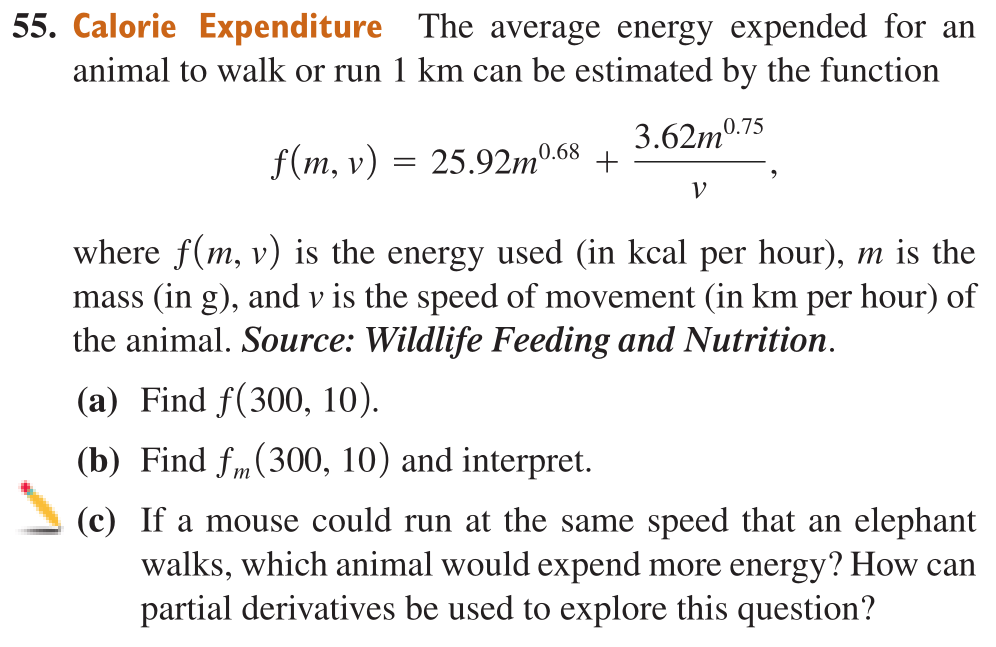
\includegraphics[width=.83\textwidth]{screenshots/55.png}
            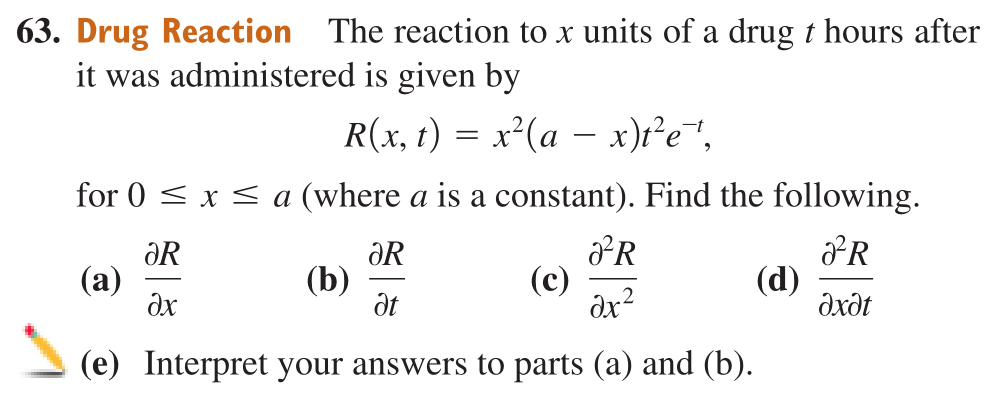
\includegraphics[width=.83\textwidth]{screenshots/63.png}
            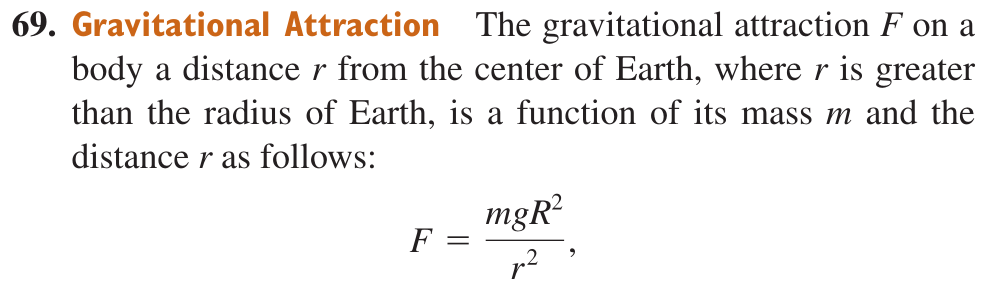
\includegraphics[width=.83\textwidth]{screenshots/69-1.png}
            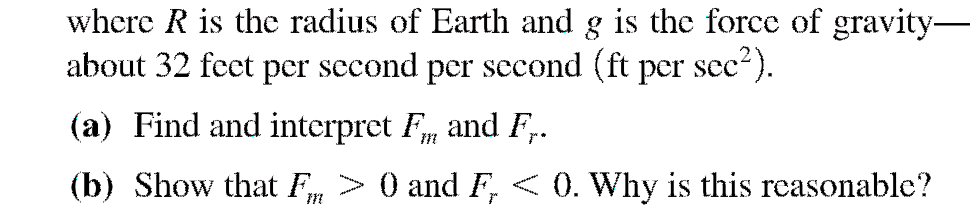
\includegraphics[width=.83\textwidth]{screenshots/69-2.png}
        \end{center}

        \newpage

    \item 
        (\textsc{\textcolor{magenta}{Submit}})
        \begin{center}
            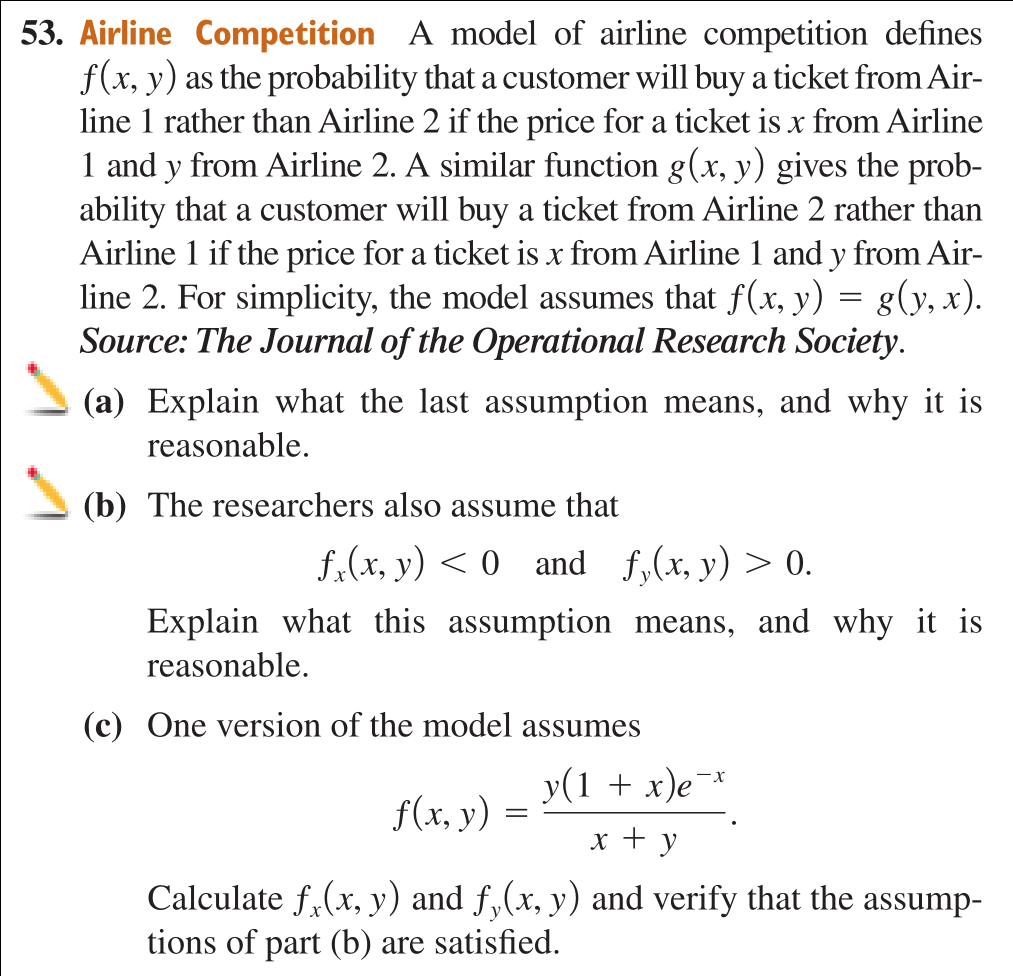
\includegraphics[width=.83\textwidth]{screenshots/53.png}
        \end{center}

    \item 
        (\textsc{Recreation})
        Suppose that in the $2$-dimensional plane ($\Reals^2$),
        every point is to be colored either red or blue.
        Show that no matter how the points in the plane are colored,
        there has to exist some equilateral triangle in the plane 
        such that the vertices of the triangle are all the same color.

\end{enumerate}

\end{document}

